\documentclass[10pt,landscape]{article}
\usepackage{multicol}
\usepackage{calc}
\usepackage{ifthen}
\usepackage{gensymb}
\usepackage[landscape]{geometry}
\usepackage{float} % for keeping figures in place \begin{figure}[H]
\usepackage{hyperref}
\usepackage{tikz} % for rainbow method in expansion
\usetikzlibrary{calc,shapes} % for rainbow method in expansion
\usetikzlibrary{quotes,angles} % for angles
\usepackage{pstricks-add} % for geogebra
\usepackage{amsmath,amssymb}
\usepackage{fancyhdr}
\usepackage{tabularx,array,booktabs} % for stretching tables to page width
\newcolumntype{Y}{>{\centering\arraybackslash}X} % for centering tables in tabularx
\newcolumntype{N}{@{}m{0pt}@{}} % for vertical space in tabularx
\newcommand{\heading}[1]{\bfseries\begin{tabular}{@{}c@{}} #1 \end{tabular}} % for a header in tables
\def\tabularxcolumn#1{m{#1}} % for vertically centering text in tables

\linespread{1.2}

\newenvironment{framed}
{
 \begin{center}
}
{
\end{center} 
}



\newenvironment{cfbox}
{
\begin{center}\fbox
}
{
\end{center}
}

\newenvironment{Figure}
  {\par\medskip\noindent\minipage{\linewidth}}
  {\endminipage\par\medskip}





% This sets page margins to .5 inch if using letter paper, and to 1cm
% if using A4 paper. (This probably isn't strictly necessary.)
% If using another size paper, use default 1cm margins.
\ifthenelse{\lengthtest { \paperwidth = 11in}}
	{ \geometry{top=.5in,left=.5in,right=.5in,bottom=.7in} }
	{\ifthenelse{ \lengthtest{ \paperwidth = 297mm}}
		{\geometry{top=1cm,left=1cm,right=1cm,bottom=1cm} }
		{\geometry{top=1cm,left=1cm,right=1cm,bottom=1cm} }
	}

% Turn off header and footer
%\pagestyle{empty}


 

% Redefine section commands to use less space
\makeatletter
\renewcommand{\section}{\@startsection{section}{1}{0mm}%
                                {-1ex plus -.5ex minus -.2ex}%
                                {0.5ex plus .2ex}%x
                                {\normalfont\large\bfseries}}
\renewcommand{\subsection}{\@startsection{subsection}{2}{0mm}%
                                {-1explus -.5ex minus -.2ex}%
                                {0.5ex plus .2ex}%
                                {\normalfont\normalsize\bfseries}}
\renewcommand{\subsubsection}{\@startsection{subsubsection}{3}{0mm}%
                                {-1ex plus -.5ex minus -.2ex}%
                                {1ex plus .2ex}%
                                {\normalfont\small\bfseries}}
\makeatother

% Define BibTeX command
\def\BibTeX{{\rm B\kern-.05em{\sc i\kern-.025em b}\kern-.08em
    T\kern-.1667em\lower.7ex\hbox{E}\kern-.125emX}}

% Don't print section numbers
%\setcounter{secnumdepth}{0}
\setcounter{secnumdepth}{1}


\setlength{\parindent}{0pt}
\setlength{\parskip}{0pt plus 0.5ex}


\pagestyle{fancy}
\fancyhf{} % sets both header and footer to nothing
\renewcommand{\headrulewidth}{0pt}
\lfoot{\sc{\copyright\ 2019 Eugene Guo Youjun\\All rights reserved}}
\cfoot{\sc{Page \thepage}}
\rfoot{\sc{For Hai Sing Catholic School}}

% -----------------------------------------------------------------------

\begin{document}

\raggedright
\footnotesize
\begin{multicols}{3}


% multicol parameters
% These lengths are set only within the two main columns
\setlength{\columnseprule}{0.25pt}
\setlength{\premulticols}{1pt}
\setlength{\postmulticols}{1pt}
\setlength{\multicolsep}{1pt}
\setlength{\columnsep}{2pt}

\begin{center}
     \Large{\textbf{Elementary Mathematics Notes (Diagrams)}} \\
    \small{Reproduced from \url{http://teach.sg}}
\end{center}


\section{Angles, Triangles \& Polygons}


\subsection{Names of angles}
\begin{minipage}{0.15\textwidth}
\begin{figure}[H]
\centering
\begin{tikzpicture}[xscale=0.5, yscale=0.5]
  \draw [line width =0.8pt]
    (3,0) coordinate (a) 
    -- (0,0) coordinate (b) 
    -- (0,3) coordinate (c) ;
       \draw [line width =0.8pt] (0,15pt) -- ++(15pt,0) -- ++(0,-15pt);
\end{tikzpicture}
\leavevmode\\
right angle\\
$(90\degree)$
\end{figure}
\end{minipage}
\begin{minipage}{0.15\textwidth}
\begin{figure}[H]
\centering
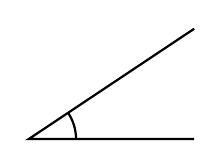
\begin{tikzpicture}[xscale=0.7, yscale=0.7]
  \draw [line width =0.8pt]
    (3,0) coordinate (a) 
    -- (0,0) coordinate (b) 
    -- (3,2) coordinate (c) 
    pic[draw=black, -, angle eccentricity=1.2, angle radius=0.6cm]
    {angle=a--b--c};
\end{tikzpicture}
\leavevmode\\
acute angle\\
$(<90\degree)$
\end{figure}
\end{minipage}
\begin{minipage}{0.15\textwidth}
\begin{figure}[H]
\centering
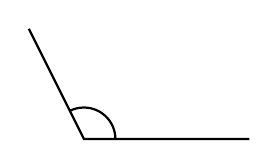
\begin{tikzpicture}[xscale=0.7, yscale=0.7]
  \draw [line width =0.8pt]
    (3,0) coordinate (a) 
    -- (0,0) coordinate (b) 
    -- (-1,2) coordinate (c) 
    pic[draw=black, -, angle eccentricity=1.2, angle radius=0.4cm]
    {angle=a--b--c};
\end{tikzpicture}
\leavevmode\\
obtuse angle\\
($90\degree <\theta< 180\degree$)
\end{figure}
\end{minipage}
\begin{minipage}{0.15\textwidth}
\begin{figure}[H]
\centering
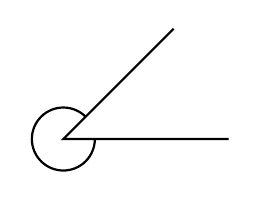
\begin{tikzpicture}[xscale=0.7, yscale=0.7]
  \draw [line width =0.8pt]
    (2,2) coordinate (a) 
    -- (0,0) coordinate (b) 
    -- (3,0) coordinate (c) 
    pic[draw=black, -, angle eccentricity=1.2, angle radius=0.4cm]
    {angle=a--b--c};
\end{tikzpicture}
\leavevmode\\
reflex angle\\
($180\degree<\theta< 360\degree$)
\end{figure}
\end{minipage}



\subsection{Types of angles}


\begin{figure}[H]
\centering
\psset{xunit=1.0cm,yunit=1.0cm,algebraic=true,dimen=middle,dotstyle=o,dotsize=3pt 0,linewidth=0.8pt,arrowsize=3pt 2,arrowinset=0.25}
\begin{pspicture*}(-4.4,3.5)(2,5.5)
\psline(-1.21,3.59)(-2.55025281714,5.35050274345)
\rput[tl](-0.8,4.3){$b$}
\rput[tl](-2.2,4.0){$a$}
\psline(-1.21,3.59)(-3.77,3.59)
\pscustom[linecolor=black,fillcolor=white,fillstyle=solid,opacity=0.1]{
\parametricplot{2.2214838521628373}{3.141592653589793}{0.703591773639*cos(t)+-1.21|0.703591773639*sin(t)+3.59}
\lineto(-1.21,3.59)\closepath}
\psline(-1.21,3.59)(1.35,3.59)
\pscustom[linecolor=black,fillcolor=white,fillstyle=solid,opacity=0.1]{
\parametricplot{0.0}{2.2214838521628373}{0.469061182426*cos(t)+-1.21|0.469061182426*sin(t)+3.59}\lineto(-1.21,3.59)\closepath}
\end{pspicture*}
\end{figure}
\begin{center}$\angle$ on a st. line\end{center}


\begin{figure}[H]
\centering
\psset{xunit=0.8cm,yunit=0.8cm,algebraic=true,dimen=middle,dotstyle=o,dotsize=3pt 0,linewidth=0.8pt,arrowsize=3pt 2,arrowinset=0.25}
\begin{pspicture*}(-7,2)(6,6)
\psline(-1.68248962965,0.964780687771)(-1.49486515668,4.17784978739)
\psline(-1.49486515668,4.17784978739)(-2.99586094044,7.15638829579)
\psline(-1.49486515668,4.17784978739)(2.82049772164,4.52964567421)
\pscustom[linecolor=black,fillcolor=white,fillstyle=solid,opacity=0.1]{
\parametricplot{0.08134186360997461}{2.0375885795181468}{0.703591773639*cos(t)+-1.49486515668|0.703591773639*sin(t)+4.17784978739}
\lineto(-1.49486515668,4.17784978739)\closepath}
\pscustom[linecolor=black,fillcolor=white,fillstyle=solid,opacity=0.1]{
\parametricplot{2.0375885795181468}{4.6540610566586835}{0.469061182426*cos(t)+-1.49486515668|0.469061182426*sin(t)+4.17784978739}
\lineto(-1.49486515668,4.17784978739)\closepath}
\rput[tl](-1.1,5.3){$x$}
\rput[tl](-2.4,4.){$z$}
\pscustom[linecolor=black,fillcolor=white,fillstyle=solid,opacity=0.1]{
\parametricplot{-1.6291242505209031}{0.08134186360997475}{0.586326478032*cos(t)+-1.49486515668|0.586326478032*sin(t)+4.17784978739}
\lineto(-1.49486515668,4.17784978739)\closepath}
\rput[tl](-0.95,3.6){$y$}
\end{pspicture*}
\end{figure}
\begin{center}$\angle$ at a pt.\end{center}






\begin{figure}[H]
\centering
\psset{xunit=0.9cm,yunit=0.9cm,algebraic=true,dimen=middle,dotstyle=o,dotsize=3pt 0,linewidth=0.8pt,arrowsize=3pt 2,arrowinset=0.25}
\begin{pspicture*}(-4.4,2)(2,5.5)
\psline(-0.978897856013,3.82605390057)(1.47821305384,0.983513828384)
\psline(-0.978897856013,3.82605390057)(-3.37110988638,6.59351487688)
\psline(-3.76981189145,0.824062333043)(-0.978897856013,3.82605390057)
\psline(-0.978897856013,3.82605390057)(1.37069633031,6.35334848754)
\pscustom[linecolor=black,fillcolor=white,fillstyle=solid,opacity=0.1]{
\parametricplot{0.8218192976119527}{2.283595036461853}{0.469061182426*cos(t)+-0.978897856013|0.469061182426*sin(t)+3.82605390057}
\lineto(-0.978897856013,3.82605390057)\closepath}
\pscustom[linecolor=black,fillcolor=white,fillstyle=solid,opacity=0.1]{
\parametricplot{-2.3197733559778406}{-0.8579976171279402}{0.469061182426*cos(t)+-0.978897856013|0.469061182426*sin(t)+3.82605390057}
\lineto(-0.978897856013,3.82605390057)\closepath}
\pscustom[linecolor=black,fillcolor=white,fillstyle=solid,opacity=0.1]{
\parametricplot{2.283595036461853}{3.9634119512017465}{0.234530591213*cos(t)+-0.978897856013|0.234530591213*sin(t)+3.82605390057}
\lineto(-0.978897856013,3.82605390057)\closepath}
\pscustom[linecolor=black,fillcolor=white,fillstyle=solid,opacity=0.1]{
\parametricplot{-0.8579976171279402}{0.8218192976119527}{0.234530591213*cos(t)+-0.978897856013|0.234530591213*sin(t)+3.82605390057}
\lineto(-0.978897856013,3.82605390057)\closepath}
\pscustom[linecolor=black,fillcolor=white,fillstyle=solid,opacity=0.1]{
\parametricplot{2.283595036461853}{3.9634119512017465}{0.351795886819*cos(t)+-0.978897856013|0.351795886819*sin(t)+3.82605390057}
\lineto(-0.978897856013,3.82605390057)\closepath}
\pscustom[linecolor=black,fillcolor=white,fillstyle=solid,opacity=0.1]{
\parametricplot{-0.8579976171279402}{0.8218192976119527}{0.351795886819*cos(t)+-0.978897856013|0.351795886819*sin(t)+3.82605390057}
\lineto(-0.978897856013,3.82605390057)\closepath}
\end{pspicture*}
\end{figure}
\begin{center}vert. opp. $\angle$\end{center}

\begin{figure}[H]
\centering
\psset{xunit=0.5cm,yunit=0.5cm,algebraic=true,dimen=middle,dotstyle=o,dotsize=3pt 0,linewidth=0.8pt,arrowsize=3pt 2,arrowinset=0.25}
\begin{pspicture*}(-4.4,0.5)(2,7)
\psline[ArrowInside=->](-3.72,6.08)(1.81,6.08)
\psline(1.81,6.08)(-4.1,0.9)
\psline(-4.1,0.9)(3.06,0.9)
\psline(-3.72,6.08)(1.81,6.08)
\psline[ArrowInside=->](-4.1,0.9)(3.06,0.9)
\pscustom[linecolor=black,fillcolor=white,fillstyle=solid,opacity=0.1]{
\parametricplot{0.0}{0.7196679213790743}{0.703591773639*cos(t)+-4.1|0.703591773639*sin(t)+0.9}
\lineto(-4.1,0.9)\closepath}
\pscustom[linecolor=black,fillcolor=white,fillstyle=solid,opacity=0.1]{
\parametricplot{3.141592653589793}{3.8612605749688673}{0.703591773639*cos(t)+1.81|0.703591773639*sin(t)+6.08}
\lineto(1.81,6.08)\closepath}
\end{pspicture*}
\end{figure}

\begin{center}alt. $\angle$\end{center}


\begin{figure}[H]
\centering
\psset{xunit=0.3cm,yunit=0.3cm,algebraic=true,dimen=middle,dotstyle=o,dotsize=3pt 0,linewidth=0.8pt,arrowsize=3pt 2,arrowinset=0.25}
\begin{pspicture*}(-4.4,-1.3)(6,9.3)
\psline(-4.26356681875,-3.27658483189)(-2.02,3.49)
\psline(-2.02,3.49)(-0.191734378467,9.00403877073)
\psline[ArrowInside=->](-0.191734378467,9)(7.54,9.)
\psline[ArrowInside=->](-2.02,3.49)(6.87,3.49)
\psline(-4.26356681875,-3.27658483189)(-0.191734378467,9.00403877073)
\psline(6.87,3.49)(-2.02,3.49)
\pscustom[linecolor=black,fillcolor=white,fillstyle=solid,opacity=0.1]{
\parametricplot{-1.8909550862281845}{0.0}{0.590102984364*cos(t)+-2.02|0.590102984364*sin(t)+3.49}
\lineto(-2.02,3.49)\closepath}
\pscustom[linecolor=black,fillcolor=white,fillstyle=solid,opacity=0.1]{
\parametricplot{-1.8909550862281845}{-5.223627931225661E-4}{0.590102984364*cos(t)+-0.191734378467|0.590102984364*sin(t)+9.00403877073}
\lineto(-0.191734378467,9.00403877073)\closepath}
\end{pspicture*}
\end{figure}


\begin{center}corr. $\angle$\end{center}


\psset{xunit=0.8cm,yunit=0.8cm,algebraic=true,dimen=middle,dotstyle=o,dotsize=5pt 0,linewidth=0.8pt,arrowsize=3pt 2,arrowinset=0.25}
\begin{pspicture*}(-4.3,-0.16)(7.3,3.3)
\psline(-1.,3.)(3.,3.)
\psline(-1.,3.)(-3.,0.)
\psline(-3.,0.)(2.,0.)
\pscustom[linecolor=black,fillcolor=white,fillstyle=solid,opacity=0.1]{
\parametricplot{0.0}{0.982793723247329}{0.5*cos(t)+-3.|0.5*sin(t)+0.}
\lineto(-3.,0.)\closepath}
\pscustom[linecolor=black,fillcolor=white,fillstyle=solid,opacity=0.1]{
\parametricplot{-2.1587989303424644}{0.0}{0.3*cos(t)+-1.|0.3*sin(t)+3.}
\lineto(-1.,3.)\closepath}
\psline{->}(-1.,3.)(1.,3.)
\psline{->}(-3.,0.)(-0.44,0.)
\begin{scriptsize}
\rput[tl](-0.84,2.62){$a$}
\rput[tl](-2.37,0.47){$b$}
\rput[tl](-0.72,1.44){$a+b=180\degree$}
\end{scriptsize}
\end{pspicture*}

\begin{center}int. $\angle$\end{center}



\section{Mensuration}


\subsection{Perimeter \& area}

\subsubsection{Parallelogram} 

\begin{figure}[H]
\centering
\psset{xunit=1.1cm,yunit=1.1cm,algebraic=true,dimen=middle,dotstyle=o,dotsize=3pt 0,linewidth=0.8pt,arrowsize=3pt 2,arrowinset=0.25}
\begin{pspicture*}(-3,-0.49)(7.3,2.3)
\psline(-0.725942746287,2.02755332682)(2.67405725371,2.02755332682)
\psline(-1.42408140081,0.122216582178)(1.97591859919,0.122216582178)
\psline(-0.725942746287,2.02755332682)(-1.42408140081,0.122216582178)
\psline(1.97591859919,0.122216582178)(2.67405725371,2.02755332682)
\psline(-1.43862595611,-0.139585413268)(1.96137404389,-0.139585413268)
\psline{<->}(-1.43862595611,-0.139585413268)(1.96137404389,-0.139585413268)
\psline(2.89565152405,2.01300877151)(2.9,0.12)
\psline{<->}(2.89565152405,2.01300877151)(2.9,0.119999999997)
\rput[tl](-0.0132595364606,-0.255941855688){$b$}
\rput[tl](2.96837430057,1.21305822987){$h$}
\end{pspicture*}
\end{figure}

Area = $b\times h$

\subsubsection{Trapezium} 

\begin{figure}[H]
\centering
\psset{xunit=0.75cm,yunit=0.75cm,algebraic=true,dimen=middle,dotstyle=o,dotsize=3pt 0,linewidth=0.8pt,arrowsize=3pt 2,arrowinset=0.25}
\begin{pspicture*}(-4.06666666667,-1.3325)(7.73333333333,3.2875)
\pspolygon[linecolor=black,fillcolor=white,fillstyle=solid,opacity=0.1](-2.08666666667,-0.3325)(4.07333333333,-0.3325)(2.85333333333,2.2675)(-0.746666666667,2.2675)
\psline[linecolor=black](-2.08666666667,-0.3325)(4.07333333333,-0.3325)
\psline[linecolor=black](4.07333333333,-0.3325)(2.85333333333,2.2675)
\psline[linecolor=black](2.85333333333,2.2675)(-0.746666666667,2.2675)
\psline[linecolor=black](-0.746666666667,2.2675)(-2.08666666667,-0.3325)
\psline(-0.746666666667,2.5875)(2.87333333333,2.5875)
\psline(4.39333333333,-0.3325)(4.39333333333,2.2475)
\psline(-2.08666666667,-0.7325)(4.09333333333,-0.7325)
\psline{<->}(-2.08666666667,-0.7325)(4.09333333333,-0.7325)
\psline{<->}(4.39333333333,-0.3325)(4.39333333333,2.2475)
\psline{<->}(2.87333333333,2.5875)(-0.74666666667,2.5875)
\rput[tl](0.833333333333,3.0275){$a$}
\rput[tl](0.673333333333,-0.9125){$b$}
\rput[tl](4.53333333333,1.0075){$h$}
\end{pspicture*}
\end{figure}

Area = $\dfrac{a+b}{2} \times h$\\[\baselineskip]

\subsubsection{Circle} 

\begin{figure}[H]
\centering
\psset{xunit=0.75cm,yunit=0.75cm,algebraic=true,dimen=middle,dotstyle=o,dotsize=3pt 0,linewidth=0.8pt,arrowsize=3pt 2,arrowinset=0.25}
\begin{pspicture*}(-4.3,-0.7)(7.3,3.8)
\pscircle[linewidth=1pt](0.88,1.58){1.67255045}
\psline[linewidth=1pt](0.88,1.58)(2.91622746827,2.48938314117)
\rput[tl](1.62,2.56){$r$}
\rput[tl](0.4,1.5){$O$}
\psdots[dotstyle=*,linecolor=black](0.88,1.58)
\end{pspicture*}
\end{figure}


Circumference = $2\pi r$\\
Area = $\pi r^2$


\subsection{Surface area \& volume}

\subsubsection{Cuboid}

\begin{figure}[H]
\centering
\psset{xunit=0.4cm,yunit=0.4cm,algebraic=true,dimen=middle,dotstyle=o,dotsize=3pt 0,linewidth=0.8pt,arrowsize=3pt 2,arrowinset=0.25}
\begin{pspicture}(0,-3.17375)(9.48,3.15375)
\psline[linewidth=0.8pt](0.0,1.39375)(7.12,1.35375)
\psline[linewidth=0.8pt](7.14,1.41375)(7.16,-2.60625)
\psline[linewidth=0.8pt](0.04,-2.60625)(7.18,-2.60625)
\psline[linewidth=0.8pt](0.04,1.35375)(0.06,-2.66625)
\psline[linewidth=0.8pt](2.3,3.13375)(0.02,1.41375)
\psline[linewidth=0.8pt](9.4,3.09375)(7.12,1.37375)
\psline[linewidth=0.8pt](9.44,-0.88625)(7.16,-2.60625)
\psline[linewidth=0.8pt](9.44,3.11375)(9.46,-0.90625)
\usefont{T1}{ptm}{m}{n}
\rput(3.6414063,-3.19625){$l$}
\usefont{T1}{ptm}{m}{n}
\rput(6.611406,-0.43625){$h$}
\psline[linewidth=0.8pt](2.3,3.13375)(9.42,3.09375)
\usefont{T1}{ptm}{m}{n}
\rput(8.631406,-2.23625){$b$}
\end{pspicture} 
\end{figure}

Surface area = $2 (lb + lh + bh)$\\
Volume = $l \times b \times h$


\subsubsection{Cylinder}

\begin{figure}[H]
\centering
\psset{xunit=0.4cm,yunit=0.4cm,algebraic=true,dimen=middle,dotstyle=o,dotsize=3pt 0,linewidth=0.8pt,arrowsize=3pt 2,arrowinset=0.25}
\begin{pspicture}(0,-3.63)(5.761875,3.61)
\psellipse[linewidth=0.8pt,dimen=outer](2.56,3.03)(2.54,0.58)
\psline[linewidth=0.8pt](0.04,3.01)(0.02,-2.83)
\psline[linewidth=0.8pt](5.08,3.07)(5.06,-2.77)
\psbezier[linewidth=0.8pt](0.0,-2.81)(0.0,-3.61)(5.08,-3.53)(5.08,-2.73)
\psbezier[linewidth=0.8pt,linestyle=dashed,dash=0.16cm 0.16cm](0.04,-2.79)(0.04,-1.99)(5.04,-1.99)(5.04,-2.79)
\psline[linewidth=0.8pt](2.48,-2.81)(5.06,-2.79)
\usefont{T1}{ptm}{m}{n}
\rput(5.5514065,0.2){$h$}
\usefont{T1}{ptm}{m}{n}
\rput(3.4614062,-2.56){$r$}
\end{pspicture} 
\end{figure}

Surface area = 2 $\times$ base area + curved surface area \\
= $2 \pi r^2 + 2 \pi r h$\\
Volume = base area $\times$ height \\
= $\pi r^2 h$



\subsubsection{Prism}


\begin{figure}[H]
\centering
\psset{xunit=0.6cm,yunit=0.6cm,algebraic=true,dimen=middle,dotstyle=o,dotsize=3pt 0,linewidth=0.8pt,arrowsize=3pt 2,arrowinset=0.25}
\begin{pspicture}(0,-1.2)(9.58,1.22)
\psline[linewidth=0.8pt](1.26,1.18)(8.24,1.18)
\psline[linewidth=0.8pt](9.54,-1.14)(8.24,1.2)
\psline[linewidth=0.8pt](2.48,-1.18)(9.56,-1.18)
\psline{<->}(0,-1.5)(9.56,-1.5)
\rput(4.5,-2){$l$}
\psline[linewidth=0.8pt,linestyle=dashed,dash=0.16cm 0.16cm](8.22,1.2)(7.46,-0.5)
\psline[linewidth=0.8pt,linestyle=dashed,dash=0.16cm 0.16cm](9.52,-1.16)(7.46,-0.5)
\psline[linewidth=0.8pt,linestyle=dashed,dash=0.16cm 0.16cm](7.46,-0.48)(2.2,-0.48)
\pstriangle[linewidth=0.8pt,dimen=outer,fillstyle=solid,fillcolor=lightgray](1.26,-1.2)(2.52,2.4)
\end{pspicture} 
\end{figure}

Volume = cross-sectional area $\times$ $l$ 

\subsubsection{Pyramid}


\begin{figure}[H]
\centering
\psset{xunit=0.6cm,yunit=0.6cm,algebraic=true,dimen=middle,dotstyle=o,dotsize=3pt 0,linewidth=0.8pt,arrowsize=3pt 2,arrowinset=0.25}
\begin{pspicture}(0,-2.2)(8.5,2.2)
\psline[linewidth=0.04cm](0.0,-2.06)(2.0,1.98)
\psline[linewidth=0.04cm](2.0,1.98)(3.6,-2.14)
\psline[linewidth=0.04cm](3.6,-2.14)(0.0,-2.06)
\psline[linewidth=0.04cm,linestyle=dashed,dash=0.16cm 0.16cm](0.02,-2.08)(1.78,-1.08)
\psline[linewidth=0.04cm,linestyle=dashed,dash=0.16cm 0.16cm](1.78,-1.08)(3.58,-2.12)
\psline[linewidth=0.04cm,linestyle=dashed,dash=0.16cm 0.16cm](1.78,-1.08)(2.02,1.94)
\psline[linewidth=0.04cm,linestyle=dashed,dash=0.16cm 0.16cm](5.12,-2.12)(6.46,-0.86)
\psline[linewidth=0.04cm,linestyle=dashed,dash=0.16cm 0.16cm](6.46,-0.86)(8.42,-0.88)
\psline[linewidth=0.04cm,linestyle=dashed,dash=0.16cm 0.16cm](6.44,-0.88)(6.46,2.18)
\psline[linewidth=0.04cm](8.48,-0.9)(7.26,-2.14)
\psline[linewidth=0.04cm](7.26,-2.14)(5.14,-2.14)
\psline[linewidth=0.04cm](5.14,-2.14)(6.46,2.18)
\psline[linewidth=0.04cm](6.46,2.18)(7.24,-2.18)
\psline[linewidth=0.04cm](8.48,-0.92)(6.48,2.16)
\end{pspicture} 
\end{figure}


Volume = $\frac{1}{3} \times$ base area $\times$ height 

\subsubsection{Cone}

\begin{figure}[H]
\centering
\psset{xunit=0.6cm,yunit=0.6cm,algebraic=true,dimen=middle,dotstyle=o,dotsize=3pt 0,linewidth=0.8pt,arrowsize=3pt 2,arrowinset=0.25}
\begin{pspicture}(0,-3.25)(6.681875,3.25)
\psbezier[linewidth=0.04](0.32,-2.43)(0.32,-3.23)(5.56,-3.23)(5.56,-2.43)
\psbezier[linewidth=0.04,linestyle=dashed,dash=0.16cm 0.16cm](5.56,-2.41)(5.56,-1.61)(0.32,-1.61)(0.32,-2.41)
\psline[linewidth=0.04cm](0.32,-2.47)(2.86,3.11)
\psline[linewidth=0.04cm](2.86,3.11)(5.56,-2.33)
\psline[linewidth=0.04cm](2.96,-2.39)(5.54,-2.37)
\psline[linewidth=0.04cm,arrowsize=0.05291667cm 2.0,arrowlength=1.4,arrowinset=0.4]{<->}(5.9,3.23)(5.9,-2.49)
\usefont{T1}{ptm}{m}{n}
\rput(4.041406,-2.16){$r$}
\usefont{T1}{ptm}{m}{n}
\rput(6.371406,0.72){$h$}
\usefont{T1}{ptm}{m}{n}
\rput(0.88140625,0.46){$l$}
\psline[linewidth=0.04cm,arrowsize=0.05291667cm 2.0,arrowlength=1.4,arrowinset=0.4]{<->}(2.66,3.11)(0.0,-2.53)
\end{pspicture} 
\end{figure}


Volume = $\frac{1}{3} \times$ base area $\times$ height \\
= $\frac{1}{3} \pi r^2 h $\\ 
Surface Area = base area + curved surface area \\
= $\pi r^2 + \pi r l$ 


\subsubsection{Sphere}


\begin{figure}[H]
\centering
\psset{xunit=0.6cm,yunit=0.6cm,algebraic=true,dimen=middle,dotstyle=o,dotsize=3pt 0,linewidth=0.8pt,arrowsize=3pt 2,arrowinset=0.25}
\begin{pspicture}(0,-2.66)(5.32,2.66)
\psbezier[linewidth=0.04](0.04,-0.06)(0.04,-0.86)(5.28,-0.86)(5.28,-0.06)
\psbezier[linewidth=0.04,linestyle=dashed,dash=0.16cm 0.16cm](5.28,-0.04)(5.28,0.76)(0.04,0.76)(0.04,-0.04)
\psline[linewidth=0.04cm](2.68,-0.02)(5.26,0.0)
\usefont{T1}{ptm}{m}{n}
\rput(3.7614062,0.21){$r$}
\pscircle[linewidth=0.04,dimen=outer](2.66,0.0){1.596}
\end{pspicture} 
\end{figure}


Volume = $\frac{4}{3} \pi r^3 $ \\ 
Surface area = $4 \pi r^2$ 


\section{Functions \& Graphs}


\subsection{Graphs of power functions ($y=ax^n$)}

\begin{cfbox}{$n=2$}\end{cfbox}
\begin{Figure}
\centering
\psset{xunit=0.5cm,yunit=0.5cm,algebraic=true,dimen=middle,dotstyle=o,dotsize=5pt 0,linewidth=0.8pt,arrowsize=3pt 2,arrowinset=0.25}
\begin{pspicture*}(-8.8,-4.73)(8.8,4.73)
\psaxes[labelFontSize=\scriptstyle,xAxis=true,yAxis=true,labels=none,Dx=1.,Dy=1.,ticks=none]{->}(0,0)(-5.8,-4.73)(5.8,4.73)[\scriptsize{$x$},140] [\scriptsize{$y$},-40]
\rput{0.}(0.,0.){\psplot{-4.}{4.}{x^2/5/0.5}}
\rput{-180.}(0.,0.){\psplot[linestyle=dashed,dash=3pt 3pt]{-4.}{4.}{x^2/5/0.5}}
\rput[tl](-0.52,-0.17){\scriptsize{$O$}}
\rput[tl](3,2.29){\scriptsize{$a>0$: $y=x^2$}}
\rput[tl](3,-2.29){\scriptsize{$a>0$: $y=-x^2$}}
\end{pspicture*}
\end{Figure}

\begin{cfbox}{$n=3$}\end{cfbox}
\begin{Figure}
\centering
\psset{xunit=0.5cm,yunit=0.5cm,algebraic=true,dimen=middle,dotstyle=o,dotsize=5pt 0,linewidth=0.8pt,arrowsize=3pt 2,arrowinset=0.25}
\begin{pspicture*}(-8.8,-4.73)(8.8,4.73)
\psaxes[labelFontSize=\scriptstyle,xAxis=true,yAxis=true,labels=none,Dx=1.,Dy=1.,ticks=none]{->}(0,0)(-5.8,-4.73)(5.8,4.73)[\scriptsize{$x$},140] [\scriptsize{$y$},-40]
\rput{0.}(0.,0.){\psplot{-4.}{4.}{x^3/16/0.5}}
\rput{-180.}(0.,0.){\psplot[linestyle=dashed,dash=3pt 3pt]{-4.}{4.}{-x^3/16/0.5}}
\rput[tl](-0.52,-0.17){\scriptsize{$O$}}
\rput[tl](3,2.29){\scriptsize{$a>0$: $y=x^3$}}
\rput[tl](3,-2.29){\scriptsize{$a>0$: $y=-x^3$}}
\end{pspicture*}
\end{Figure}


\begin{cfbox}{$n=-2$}\end{cfbox}
\begin{Figure}
\centering
\psset{xunit=0.5cm,yunit=0.5cm,algebraic=true,dimen=middle,dotstyle=o,dotsize=5pt 0,linewidth=0.8pt,arrowsize=3pt 2,arrowinset=0.25}
\begin{pspicture*}(-8.8,-4.73)(8.8,4.73)
\psaxes[labelFontSize=\scriptstyle,xAxis=true,yAxis=true,labels=none,Dx=1.,Dy=1.,ticks=none]{->}(0,0)(-5.8,-4.73)(5.8,4.73)[\scriptsize{$x$},140] [\scriptsize{$y$},-40]
\rput{0.}(0.,0.){\psplot{-6}{-0.1}{x^(-2)/0.4+0.5}}
\rput{0.}(0.,0.){\psplot{0.1}{6}{x^(-2)/0.4+0.5}}
\rput{-180.}(0.,0.){\psplot[linestyle=dashed,dash=3pt 3pt]{-6}{-0.1}{x^(-2)/2/0.4+0.5}}
\rput{-180.}(0.,0.){\psplot[linestyle=dashed,dash=3pt 3pt]{0.1}{6}{x^(-2)/2/0.4+0.5}}
\rput[tl](-0.62,-0.17){\scriptsize{$O$}}
\rput[tl](2,2.29){\scriptsize{$a>0$: $y=\dfrac{1}{x^2}$}}
\rput[tl](2,-2.29){\scriptsize{$a<0$: $y=-\dfrac{1}{x^2}$}}
\end{pspicture*}
\end{Figure}

\begin{cfbox}{$n=-1$}\end{cfbox}
\begin{Figure}
\centering
\psset{xunit=0.5cm,yunit=0.5cm,algebraic=true,dimen=middle,dotstyle=o,dotsize=5pt 0,linewidth=0.8pt,arrowsize=3pt 2,arrowinset=0.25}
\begin{pspicture*}(-8.8,-4.73)(8.8,4.73)
\psaxes[labelFontSize=\scriptstyle,xAxis=true,yAxis=true,labels=none,Dx=1.,Dy=1.,ticks=none]{->}(0,0)(-5.8,-4.73)(5.8,4.73)[\scriptsize{$x$},140] [\scriptsize{$y$},-40]
\rput{0.}(0.,0.){\psplot{-6}{-0.1}{x^(-1)/2/0.5}}
\rput{0.}(0.,0.){\psplot{0.1}{6}{x^(-1)/2/0.5}}
\rput{0.}(0.,0.){\psplot[linestyle=dashed,dash=3pt 3pt]{-6}{-0.1}{-x^(-1)/2/0.5}}
\rput{0.}(0.,0.){\psplot[linestyle=dashed,dash=3pt 3pt]{0.1}{6}{-x^(-1)/2/0.5}}
\rput[tl](-0.62,-0.17){\scriptsize{$O$}}
\rput[tl](1,2.29){\scriptsize{$a>0$: $y=\dfrac{1}{x}$}}
\rput[tl](1,-2.29){\scriptsize{$a<0$: $y=-\dfrac{1}{x}$}}
\end{pspicture*}
\end{Figure}

\section{Exponential Function (Graphs)}


\subsection{Graphs of exponential function}

\begin{cfbox}{$y=a^x$}\end{cfbox}
\begin{Figure}
\centering
\psset{xunit=0.5cm,yunit=0.5cm,algebraic=true,dimen=middle,dotstyle=o,dotsize=5pt 0,linewidth=0.8pt,arrowsize=3pt 2,arrowinset=0.25}
\begin{pspicture*}(-8.8,-4.73)(8.8,4.73)
\psaxes[labelFontSize=\scriptstyle,xAxis=true,yAxis=true,labels=none,Dx=1.,Dy=1.,ticks=none]{->}(0,0)(-5.8,-4.73)(5.8,4.73)[\scriptsize{$x$},140] [\scriptsize{$y$},-40]
\rput{0.}(0.,0.){\psplot{-5.8}{6}{1.5^x}}
\psline(-0.3,1.)(0.3,1.)
\rput[tl](0.6,1.18){$1$}
\rput[tl](-0.62,-0.17){\scriptsize{$O$}}
\rput[tl](-5.8,1.6){\scriptsize{$y=5^x$}}
\end{pspicture*}
\end{Figure}




\section{Properties Of Circles}

\subsection{Angle properties}

\begin{Figure}
\centering
\psset{xunit=1.0cm,yunit=1.0cm,algebraic=true,dimen=middle,dotstyle=o,dotsize=5pt 0,linewidth=0.8pt,arrowsize=3pt 2,arrowinset=0.25}
\begin{pspicture*}(-2.8324269598517975,-1.056903770492757)(4.056592516211026,4.561210388434345)
\pspolygon[linecolor=black,fillcolor=white,fillstyle=solid,opacity=0.1](0.8880083863275616,-0.12049415735610663)(0.8885064512008807,0.13146771522802464)(0.6365445786167494,0.13196578010134358)(0.6360465137434304,-0.11999609248278764)
\pscircle(0.64,1.88){2.}
\psline(0.64,1.88)(0.6360465137434304,-0.11999609248278764)
\psline(-1.6448673729115613,-0.11548730282204633)(2.7592233010482357,-0.12419307580711857)
\begin{scriptsize}
\rput[tl](0.7252261166838207,2.150053571812354){$O$}
\psdots[dotstyle=*,dotsize=4pt](0.64,1.88)
\end{scriptsize}
\end{pspicture*}

tan. $\perp$ rad.
\end{Figure}
 
 
\begin{Figure}
\centering
\psset{xunit=1.0cm,yunit=1.0cm,algebraic=true,dimen=middle,dotstyle=o,dotsize=5pt 0,linewidth=0.8pt,arrowsize=3pt 2,arrowinset=0.25}
\begin{pspicture*}(-2.8,-1.16)(4.1,4)
\pspolygon[linecolor=black,fillcolor=white,fillstyle=solid,opacity=0.1](-0.2765259213670165,3.5431858062823283)(-0.08622439418393169,3.378048402716371)(0.07891300938202503,3.568349929899456)(-0.11138851780105974,3.733487333465413)
\pscircle(0.64,1.88){2.}
\begin{scriptsize}\psdots[dotstyle=*,dotsize=4pt](0.64,1.88)\end{scriptsize}
\psline(-0.11138851780105974,3.733487333465413)(-1.3008616542351985,2.362758779432761)
\psline(-1.3008616542351985,2.362758779432761)(2.580861654235198,1.3972412205672393)
\psline(-0.11138851780105974,3.733487333465413)(2.580861654235198,1.3972412205672393)
\rput[tl](0.27950942416278823,1.8293578375818431){\scriptsize{$O$}}
\end{pspicture*}

rt. $\angle$ in semicircle
\end{Figure}
 

 
\begin{Figure}
\centering
\psset{xunit=1.0cm,yunit=1.0cm,algebraic=true,dimen=middle,dotstyle=o,dotsize=5pt 0,linewidth=0.8pt,arrowsize=3pt 2,arrowinset=0.25}
\begin{pspicture*}(-2.8,-1.16)(4.1,4)
\pscircle(0.64,1.88){2.}
\psline(2.033368561451729,0.4452442535546546)(2.1383923028002076,3.20469638291538)
\psline(2.1383923028002076,3.20469638291538)(-0.6309354310595386,0.33574512140077584)
\pscustom[linecolor=black,fillcolor=white,fillstyle=solid,opacity=0.1]{
\parametricplot{-2.3385271909611403}{-1.6088376010180994}{0.35632859358945645*cos(t)+2.1383923028002076|0.35632859358945645*sin(t)+3.20469638291538}
\lineto(2.1383923028002076,3.20469638291538)\closepath}
\psline(2.033368561451729,0.4452442535546546)(-0.7362709936544699,3.3311644124720456)
\psline(-0.7362709936544699,3.3311644124720456)(-0.6309354310595386,0.33574512140077584)
\pscustom[linecolor=black,fillcolor=white,fillstyle=solid,opacity=0.1]{
\parametricplot{-1.5356452628945378}{-0.8059556729514971}{0.35632859358945645*cos(t)+-0.7362709936544699|0.35632859358945645*sin(t)+3.3311644124720456}
\lineto(-0.7362709936544699,3.3311644124720456)\closepath}
\end{pspicture*}

$\angle$s in same seg.
\end{Figure}
 
 
\begin{Figure}
\centering
\psset{xunit=1.0cm,yunit=1.0cm,algebraic=true,dimen=middle,dotstyle=o,dotsize=5pt 0,linewidth=0.8pt,arrowsize=3pt 2,arrowinset=0.25}
\begin{pspicture*}(-2.8,-1.16)(4.1,4)
\pscircle(0.64,1.88){2.}
\psline(-0.6309354310595386,0.33574512140077584)(0.64,1.88)
\psline(0.64,1.88)(2.033368561451729,0.4452442535546546)
\psline(2.033368561451729,0.4452442535546546)(0.9483262275697846,3.8560908221518018)
\psline(0.9483262275697846,3.8560908221518018)(-0.6309354310595386,0.33574512140077584)
\begin{scriptsize}\psdots[dotstyle=*,dotsize=4pt](0.64,1.88)\end{scriptsize}
\pscustom[linecolor=black,fillcolor=white,fillstyle=solid,opacity=0.1]{
\parametricplot{-2.259410445084871}{-0.8000312651987895}{0.35632859358945645*cos(t)+0.64|0.35632859358945645*sin(t)+1.88}
\lineto(0.64,1.88)\closepath}
\parametricplot[linecolor=black]{-2.259410445084871}{-0.8000312651987895}{0.35632859358945645*cos(t)+0.64|0.35632859358945645*sin(t)+1.88}
\parametricplot[linecolor=black]{-2.259410445084871}{-0.8000312651987895}{0.29694049465788036*cos(t)+0.64|0.29694049465788036*sin(t)+1.88}
\pscustom[linecolor=black,fillcolor=white,fillstyle=solid,opacity=0.1]{
\parametricplot{-1.9924935786257407}{-1.2628039886826998}{0.35632859358945645*cos(t)+0.9483262275697846|0.35632859358945645*sin(t)+3.8560908221518018}
\lineto(0.9483262275697846,3.8560908221518018)\closepath}
\rput[tl](0.5051842001027776,2.20944167074393){\scriptsize{$O$}}
\end{pspicture*}

$\angle$ at centre = 2 $\angle$ at circ.
\end{Figure}
 

\begin{Figure}
\centering
\psset{xunit=1.0cm,yunit=1.0cm,algebraic=true,dimen=middle,dotstyle=o,dotsize=5pt 0,linewidth=0.8pt,arrowsize=3pt 2,arrowinset=0.25}
\begin{pspicture*}(-2.8,-1.16)(4.1,4)
\pscircle(0.64,1.88){2.}
\psline(0.2757508765609353,-0.08655093401464509)(2.569477724250156,2.4064178108902086)
\psline(-0.570411696359829,3.4721380358861227)(-1.2936704347449144,1.3691980327040494)
\psline(-0.570411696359829,3.4721380358861227)(2.569477724250156,2.4064178108902086)
\psline(0.2757508765609353,-0.08655093401464509)(-1.2936704347449144,1.3691980327040494)
\pscustom[linecolor=black,fillcolor=white,fillstyle=solid,opacity=0.1]{
\parametricplot{-1.9020510693452142}{-0.3272125060377993}{0.35632859358945645*cos(t)+-0.570411696359829|0.35632859358945645*sin(t)+3.4721380358861227}
\lineto(-0.570411696359829,3.4721380358861227)\closepath}
\pscustom[linecolor=black,fillcolor=white,fillstyle=solid,opacity=0.1]{
\parametricplot{2.8143801475519936}{3.9685909033665876}{0.35632859358945645*cos(t)+2.569477724250156|0.35632859358945645*sin(t)+2.4064178108902086}
\lineto(2.569477724250156,2.4064178108902086)\closepath}
\pscustom[linecolor=black,fillcolor=white,fillstyle=solid,opacity=0.1]{
\parametricplot{0.8269982497767946}{2.393752340059173}{0.35632859358945645*cos(t)+0.2757508765609353|0.35632859358945645*sin(t)+-0.08655093401464509}
\lineto(0.2757508765609353,-0.08655093401464509)\closepath}
\pscustom[linecolor=black,fillcolor=white,fillstyle=solid,opacity=0.1]{
\parametricplot{-0.7478403135306202}{1.2395415842445794}{0.35632859358945645*cos(t)+-1.2936704347449144|0.35632859358945645*sin(t)+1.3691980327040494}
\lineto(-1.2936704347449144,1.3691980327040494)\closepath}
\begin{scriptsize}
\rput[tl](-0.4331477630161247,3.0408750557859965){$a$}
\rput[tl](-0.8844973148961028,1.5442949627102776){$b$}
\rput[tl](0.14885560651332086,0.5465749006597985){$c$}
\rput[tl](1.871110475529027,2.363850727966028){$d$}
\end{scriptsize}
\end{pspicture*}

$\angle$s in opp. seg. ($a+c=b+d=180\degree$)
\end{Figure}
 
\begin{Figure}
\centering
\psset{xunit=0.8cm,yunit=0.8cm,algebraic=true,dimen=middle,dotstyle=o,dotsize=5pt 0,linewidth=0.8pt,arrowsize=3pt 2,arrowinset=0.25}
\begin{pspicture*}(-2.3912242746085073,-1.134997220520739)(8.975412291056243,4.377104782413491)
\pspolygon[linecolor=black,fillcolor=white,fillstyle=solid,opacity=0.1](1.3946013085375395,0.01619086305151273)(1.3369295721913161,0.21589465531906915)(1.1372257799237597,0.15822291897284574)(1.194897516269983,-0.04148087329471073)
\pspolygon[linecolor=black,fillcolor=white,fillstyle=solid,opacity=0.1](1.281586019990875,3.5533550645106513)(1.4756734868733714,3.4789394141515526)(1.5500891372324699,3.673026881034049)(1.3560016703499738,3.7474425313931476)
\pscircle(0.64,1.88){1.6}
\psdots[dotstyle=*,dotsize=4pt](0.64,1.88)
\psline(1.3560016703499738,3.7474425313931476)(6.9233958339445465,1.6128314503996237)
\psline(6.9233958339445465,1.6128314503996237)(1.194897516269983,-0.04148087329471073)
\psline(1.194897516269983,-0.04148087329471073)(0.64,1.88)
\psline(1.3560016703499738,3.7474425313931476)(0.64,1.88)
\psline(0.64,1.88)(6.9233958339445465,1.6128314503996237)
\pscustom[linecolor=black,fillcolor=white,fillstyle=solid,opacity=0.1]{
\parametricplot{2.775466713726621}{3.0990984794742653}{0.6859177237901143*cos(t)+6.9233958339445465|0.6859177237901143*sin(t)+1.6128314503996237}
\lineto(6.9233958339445465,1.6128314503996237)\closepath}
\pscustom[linecolor=black,fillcolor=white,fillstyle=solid,opacity=0.1]{
\parametricplot{3.0990984794742653}{3.4227302452219095}{0.7839059700458448*cos(t)+6.9233958339445465|0.7839059700458448*sin(t)+1.6128314503996237}
\lineto(6.9233958339445465,1.6128314503996237)\closepath}
\psline(4.2169299172377,2.8815677534369795)(4.062061021165114,2.477645841949691)
\psline(4.2169299172377,2.8815677534369795)(4.139698752147259,2.6801369908963855)
\psline(4.139698752147259,2.6801369908963855)(4.062061021165114,2.477645841949691)
\psline(3.997464103943195,0.9992676677436675)(4.0591466751072645,0.7856752885524566)
\psline(4.0591466751072645,0.7856752885524566)(4.1206445104557865,0.5727226064688725)
\begin{scriptsize}
\rput[tl](0.21928658328246562,2.0087741257816814){$O$}
\rput[tl](1.0971572920955022,-0.19569930834792745){$A$}
\rput[tl](1.2519267323604018,4.050930866477608){$B$}
\rput[tl](7.054842664443922,1.7826742863837726){$P$}
\end{scriptsize}
\end{pspicture*}
tan. from ext. pt.
\end{Figure}





\begin{figure}[H]
\centering
\begin{pspicture}(0,-1.57)(11.46,1.43)
\end{pspicture} 
\end{figure}


\end{multicols}


\section{Bisectors}


\subsection{Constructing perpendicular bisector}


\begin{figure}[H]
\centering
\begin{pspicture}(0,-1.57)(11.46,1.43)
\psline[linewidth=0.8pt](0.66,0.01)(3.16,-0.01)
\rput(0.3211621,1.075){1.}
\pscircle[linewidth=0.8pt,dimen=outer,fillstyle=solid,fillcolor=black](3.17,-0.02){0.07}
\psarc[linewidth=0.8pt](3.17,-0.12){1.43}{133.8065}{167.57405}
\rput{-270.0}(3.03,-3.27){\psarc[linewidth=0.8pt](3.15,-0.12){1.43}{100.22217}{130.68398}}
\psframe[linewidth=0.8pt,dimen=outer](3.76,1.43)(0.0,-1.57)
\rput(4.1783886,1.075){2.}
\psframe[linewidth=0.8pt,dimen=outer](7.6,1.43)(3.84,-1.57)
\psline[linewidth=0.8pt](4.34,0.03)(6.84,0.01)
\psarc[linewidth=0.8pt](6.85,-0.1){1.43}{128.29016}{162.0506}
\rput{-270.0}(6.73,-6.93){\psarc[linewidth=0.8pt](6.83,-0.1){1.43}{100.22217}{130.68398}}
\rput{-180.0}(8.7,0.08){\pscircle[linewidth=0.8pt,dimen=outer,fillstyle=solid,fillcolor=black](4.35,0.04){0.07}}
\rput{-180.0}(8.7,0.28){\psarc[linewidth=0.8pt](4.35,0.14){1.43}{127.3332}{160.60219}}
\rput{-90.0}(4.23,4.51){\psarc[linewidth=0.8pt](4.37,0.14){1.43}{100.22217}{130.68398}}
\rput(8.034961,1.075){3.}
\psframe[linewidth=0.8pt,dimen=outer](11.46,1.43)(7.7,-1.57)
\psline[linewidth=0.8pt](8.2,0.03)(10.7,0.01)
\psarc[linewidth=0.8pt](10.63,-0.1){1.43}{128.29016}{162.0506}
\rput{-270.0}(10.67,-10.87){\psarc[linewidth=0.8pt](10.77,-0.1){1.43}{100.22217}{130.68398}}
\rput{-90.0}(8.03,8.31){\psarc[linewidth=0.8pt](8.17,0.14){1.43}{100.22217}{130.68398}}
\rput{-180.0}(16.62,0.2){\psarc[linewidth=0.8pt](8.31,0.1){1.43}{127.3332}{160.60219}}
\psline[linewidth=0.8pt](9.5,1.29)(9.52,-1.27)
\end{pspicture} 
\end{figure}


\subsection{Constructing angle bisector}

\begin{figure}[H]
\centering
\begin{pspicture}(0,-0.74)(11.46,2.26)
\psline[linewidth=0.8pt](1.04,1.42)(1.98,-0.26)
\rput(0.3211621,1.905){1.}
\pscircle[linewidth=0.8pt,dimen=outer,fillstyle=solid,fillcolor=black](1.97,-0.27){0.07}
\rput{-90.0}(2.56,0.98){\psarc[linewidth=0.8pt](1.77,-0.79){1.43}{133.8065}{167.57405}}
\psarc[linewidth=0.8pt](2.03,-0.83){1.43}{100.22217}{130.68398}
\psframe[linewidth=0.8pt,dimen=outer](3.76,2.26)(0.0,-0.74)
\psline[linewidth=0.8pt](1.96,-0.32)(2.88,1.44)
\psline[linewidth=0.8pt](4.72,1.52)(5.66,-0.16)
\psarc[linewidth=0.8pt](5.71,-0.73){1.43}{100.22217}{130.68398}
\psline[linewidth=0.8pt](5.66,-0.21)(6.56,1.54)
\psdots[dotsize=0.14](5.24,0.6)
\psdots[dotsize=0.14](6.06,0.62)
\rput{-90.0}(6.22,4.84){\psarc[linewidth=0.8pt](5.53,-0.69){1.43}{133.8065}{167.57405}}
\rput{-90.0}(4.76,5.18){\psarc[linewidth=0.8pt](4.97,0.21){1.43}{133.8065}{167.57405}}
\rput(4.1783886,1.905){2.}
\psframe[linewidth=0.8pt,dimen=outer](7.6,2.26)(3.84,-0.74)
\psarc[linewidth=0.8pt](6.27,0.17){1.43}{100.22217}{130.68398}
\rput(8.034961,1.905){3.}
\psframe[linewidth=0.8pt,dimen=outer](11.46,2.26)(7.7,-0.74)
\psline[linewidth=0.8pt](8.84,1.6)(9.8,-0.06)
\psarc[linewidth=0.8pt](9.83,-0.65){1.43}{100.22217}{130.68398}
\psline[linewidth=0.8pt](9.76,-0.10)(10.68,1.62)
\rput{-90.0}(10.26,9.04){\psarc[linewidth=0.8pt](9.65,-0.61){1.43}{133.8065}{167.57405}}
\psarc[linewidth=0.8pt](10.39,0.25){1.43}{100.22217}{130.68398}
\rput{-90.0}(8.72,9.34){\psarc[linewidth=0.8pt](9.03,0.31){1.43}{133.8065}{167.57405}}
\psline[linewidth=0.8pt](9.74,1.96)(9.78,-0.5)
\end{pspicture} 
\end{figure}



\end{document}

